\chapter{Methodology}\label{chap:methods}

This section of the report will explain in detail about the steps taken in implementing the approach of this thesis, granular explanation of the methodologies , tools and libraries used for the implementation of the evaluation framework and web-interface will be described in detail. Methods contain two parts of  implementations, first is the Automatic Machine learning evaluation framework, second is the web-interface. Python\footnote{\url{https://docs.python.org/3/}} programming language version 3 was used in  both the implementations, database for the accumulation of results and DASH framework\footnote{\url{https://dash.plot.ly/}} was used in designing the web-interface

The main aim of this thesis is to evaluate the performance of the two Automatic machine learning libraries Autosklearn and Tpot, this section starts with implementation details of the main aim of this thesis that is evaluation framework followed by the web-interface implementation.

\section{Evaluation framework}

\subsection{Evaluation Criteria}
Comparison study involves many different attributes depending on the candidate considered for the comparison, in context of this thesis if we are comparing two different machine learning algorithms based on there performance. the performance metric would be the main attribute of comparison, similarly if we are trying to compare the two algorithms based on there use of CPU time and memory the main attribute of comparison would be the run time of the algorithms and the ram usage during execution. Likewise there are different methodologies of evaluation in every domain, in order to form a framework of evaluation one has to decide on these attributes or the criterion's for evaluation, one such criteria for evaluating the two machine learning libraries is the performance criteria along with the run-time of these libraries, so the main attribute here would be the performance metrics, 

Further performance metrics has several types of measurements to choose from, again it depends on the task type at hand if we are evaluating the performance of an algorithm on a supervised classification or regression task the measurements would be accuracy,f1-score for classification and rmse score for regression tasks.

\subsection{Choosing the performance metric other than accuracy}
    
 With any classification tasks the datasets contains several instances, each instance will be mapped to a class or a label also called as target variable. The value of the target variable contains the name of a particular entity where the instance belongs to that named entity, for example with the tumors dataset each instance will contain the class variable value as \blockquote{malignant} or \blockquote{benign} the target value will define where does the each instance belongs to from analyzing the features, here this is a simple classification task where if we employ a algorithm to learn from the instances and predict if the person has malignant or benign tumor, the algorithm would predict accordingly from the features available in the dataset, to measure the no of correct predictions which the algorithm makes the metric accuracy is used , model prediction accuracy is defined has the no of predictions made correctly divided by the total no of predictions made, with accuracy there is a drawback, the accuracy measure does not take into account the imbalance of class/target values. With this drawback we need to consider other performance metrics for classification task such as f1-score,precision-recall scores. The detail explanation of how accuracy and other performance metrics are measured is described in the background section of this paper.

 
    
\subsection{Autosklearn Methodology}
    
    \begin{figure}[!h]
    	\centering
    	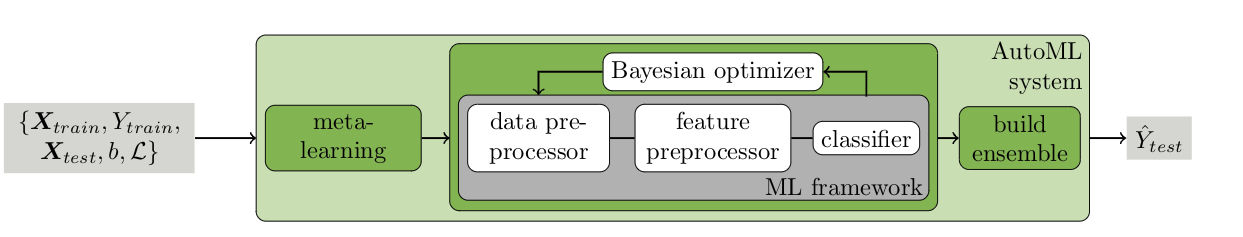
\includegraphics[width=1.1\linewidth]{thesis_template/images/autosklearn.png}
    	\caption{Autosklearn Workflow}
    	\captionsource{source:fig 1 in \cite{autosklearn}}
    	\label{fig:autosklearn_workflow}
    \end{figure}
    
The workflow of Autosklearn\footnote{\url{https://automl.github.io/auto-sklearn/stable/}} is described in the fig : \ref{fig:autosklearn_workflow} as we can see the typical ML framework is optimized with Bayesian optimizer, before the bayesian optimization process a meta-learning step to warm-start the bayesian optimizer is added as discussed in the paper \cite{autosklearn}. The meta-learning step is composed of different dataset's meta-features, these meta-features are computed from 140 datasets collected from openml platform \cite{OpenML2013}. The meta-features are computed by bayesian optimization selecting the best emperical performance from a dataset, for every dataset a ML framework instance is saved. These instances are used as a warm-start as mentioned before, the bayesian otimizer uses these instances on every run whenever a new dataset has been given, for the given dataset a certain algorithm can perform better than other algorithms, for the bayesian optimizer before the start of the optimization process certain ML instances which are saved are fed for the first round of iterations, this will give a warm start behaviour for the optimizer to look for optimal search spaces before hand.
        
The Bayesian optimizer builds a probabilistic model at first to measure the performance with a set of hyperparameters, based on this models performance the optimizer will then select optimal hyperparameter settings in the next iteration\cite{autosklearn}. In every iteration the bayesian  optimizer finds optimal hyperparameter settings based on the previous models it generated, the process continues until a threshold.
As we can see in figure \ref{autosklearn_workflow} The ML framework is wrapped with bayesian optimizer during this process several models would be trained and many of which will give best emperical performance. The next step in the work-flow is ensemble construction, the bayesian optimization process during its iterations does not save the models which may perform better than the best, due to this the ensemble step provides a great advantage. The models obtained during the bayesian optimization are saved and added to the ensemble of models, this final ensemble which consists of 100 different models from 15 algorithms and 110 hyperparameters\cite{autosklearn} each model will contain the combination of hyperparameters for its respective algorithm.
Finally the ensemble which is built is given as the end result of whole work-flow, using this ensemble we can predict with test data.
    
    
\subsection{TPOT Methodology}
    
    \begin{figure}[!h]
    	\centering
    	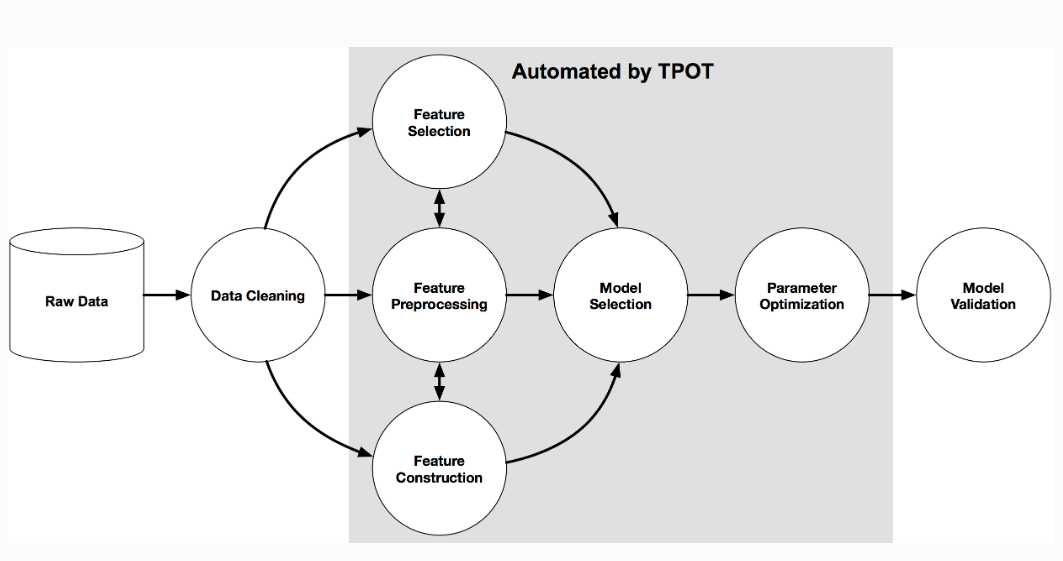
\includegraphics[width=1.1\linewidth]{thesis_template/images/tpot-git-workflow.png}
    	\caption{Tpot Automatic ML Workflow}
    	\captionsource{source: \url{https://epistasislab.github.io/tpot/}}
    	\label{fig:tpot_git_workflow}
    \end{figure}
Tree based pipeline optimization tool TPOT\cite{tpot} is a open source tool based on genetic programming, the main difference between tpot and autosklearn is the underlying algorithm configuration technique, with tpot its genetic programming and for autosklearn its bayesian optimization. Figure \ref{fig:tpot_workflow} describes the workflow of tpot. Comparing the methodology and primary aim of tpot, it produces a single best pipeline based on several generations of ML pipelines using Genetic programming and Pareto based optimization process where as autosklearn produces a ensemble consisting of 100 estimators.
Genetic programming is a well known evolutionary algorithm. Tpot uses genetic programming as implemented in DEAP\footnote{\url{https://deap.readthedocs.io/en/master/}} python package. Basic understanding of Genetic programming or genetic algorithms is  it starts of with a set of solutions to a problem which is called the initial population, the initial solutions are combined to form new solutions i.e offsprings, these new solutions are generated from technique's called as cross-over and mutation, from every mutation a better solution is generated which then again generates even better and optimal solutions. With this understanding of genetic programming, Tpot at first generates 100 solutions, each solution is a tree-based ML pipeline, these solutioins are evaluated on there balanced accuracy with Cross-validation on a given dataset. At every generation, from NSGA-II selection scheme as mentioned here\cite{tpot} tpot selects the top 20 pipelines based on there accuracy to maximize the next generations of solutions. Finally with 100 generations the process stops and produces a outcome with best optimal solution 
        
         \begin{figure}[!h]
    	\centering
    	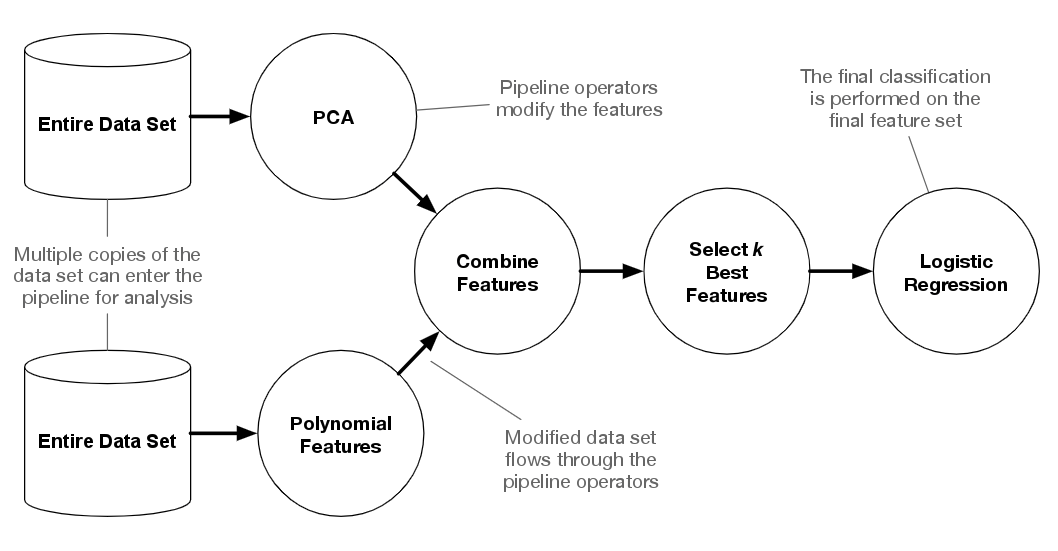
\includegraphics[width=1.0\linewidth]{thesis_template/images/tpot-workflow.png}
    	\caption{Tpot  Workflow}
    	\captionsource{source: fig 1 in \cite{tpot}}
    	\label{fig:tpot_workflow}
        \end{figure}
        
In the figure \ref{fig:tpot_workflow} we can see pipeline operators modifying the features and combining them to obtain the best features, as explained in the above section operators are treated as initial solutions which get better with generations of different combination of optimal hyperparameters. In ML sense these pipeline operators are sets of different feature engineering methods and a ML algorithm at the last step of the pipeline. At every iteration from the previous solutions they update there parameters based on scores to maximize the next outcome. This process repeats for a set of 100 generations by selecting the best operators and ignoring the degrading operators from the pile to maximize prediction accuracy at every iteration, at the end of generations tpot gives out the best pipeline as stated here \cite{tpot}
        
    
\subsection{Collection of Data sets }
The selection of datasets had to be carried out particularly for Autosklearn since it employs meta-learning where 140 of the datasets from well known data repository openml\cite{OpenML2013} has been used to generate meta-features for warm start of bayesian optimization. Considering fairness in the evaluation of the libraries, these 140 datasets had to be filtered out before considering any particular dataset. The selection of every particular dataset for the libraries upto 20 where selected out of the 140 datasets listed in this paper. \cite{autosklearn_supplementary}10 datasets of classification and regression each were obtained for each toolkit totalling to 20 datasets.
   
    
\subsection{Experiment Configuration of Autosklearn and TPOT}
In order to have fairness in the evaluation process the runtime for the libraries were set to 60 mins each with 10 fold cross validation and for future reproduction of the experiments same seed value of 2 was set for the both the toolkits
   
    
\subsection{Statisitical significance test}
Statistical significance test are used in evaluation of a ML model based on several samples of its performance scores. When comparing two models on a given dataset as in this thesis both the generated models from the toolkits are subjected to significance test in order to check if there is significant difference in there performance. Both the models are trained and tested on the same dataset for 20 repetitions with different splits, with 20 accuracy and rmse score samples obtained from the respective classification and regression tasks each, a simple hypothesis could be tested.
  
    
\section{Web Interface}
There are range of web frameworks out there for building web interfaces which aid in data analysis, visual aids such as these web interfaces allows a user to examine and find different patterns which cannot be done in console of a compiler or a Integrated Development environments (IDE). There are different categories of Visual analysis, for the context of machine learning it usually involves plots of performance, distribution, validation and learning curves of models and dataset's. In any ML workflow the first step is to analyze a dataset on its features , no of instances , the distribution of samples and classes, the no of instances and features can be shown as text but the distribution cannot be understood just by looking at the samples of data. These samples of data  will have a certain distribution, for example Gaussian Distribution\footnote{\url{https://en.wikipedia.org/wiki/Gaussian_function}} or Normal Distribution\footnote{\url{https://en.wikipedia.org/wiki/Normal_distribution}}, some algorithms perform better when there is a certain distribution present in the data samples, visualizing these distributions using different plots and charts provides a initial idea for ML practitioner to take decisions on the choice of algorithms to use before hand, these are one of the examples of how visualization facilitates and improves ML workflow. further examples include feature aggregation and creation of new features from the available features and finding interesting patterns.

The generated results from the evaluation of the autosklearn and tpot has numerous classifiers and different hyperparemeters for each run, analyzing these huge set of results just with plain text is not intuitive enough therefore a web gui with simple interface to compare the results had to be built. The interface consists of a single web page with different tabs for navigating to different sections of the page, every section contains values particular to the dataset selected and its model's results respectively, each tab is updated on the selection of a dataset from the list of names.
Keeping it as a single entry point of action and rest is built on the selection. The interface is built to describe each run of the toolkit's outcome, following the ML workflow interface starts of with a list of dataset names on selecting a name rest all the attributes and values will load up for that particular dataset. Each run of the experiments and there models parameters can be accessed.

\subsection{Choosing the web framework}
The evaluation framework being built in Python environment, the selection of web framework tool was narrowed down to be built in the same environment to ease the development of the interface and provide flexible data communication between the scripts, DASH\footnote{\url{https://dash.plot.ly/}} framweork was selected to develop the interface, since DASH framework is built using python and gives support with building graphs and charts out of the box via easy method integration's. The execution environment for evaluation framework and the web interface being the same that is Python running scripts and using the methods with each other was a advantage and saved a lot of time by cutting re implementation of certain methods and without the need of middle end communication framework. The analytical web framework provides variety of UI elements to choose from and handles layout styling with minimal bootstrap. One of the main time consuming process in creating a web-interface is the CSS\footnote{\url{https://en.wikipedia.org/wiki/Cascading_Style_Sheets}} styling which involves setting the layout dimensions and positioning the elements accordingly, with numerous UI elements handling the position of elements becomes tedious and it also has to resize accordingly to screen sizes. Since Dash provides a out of the box default layout and styling, this would save a lot of time in dealing with the styling of the layouts and UI elements.

\begin{figure}[!h]
    	\centering
    	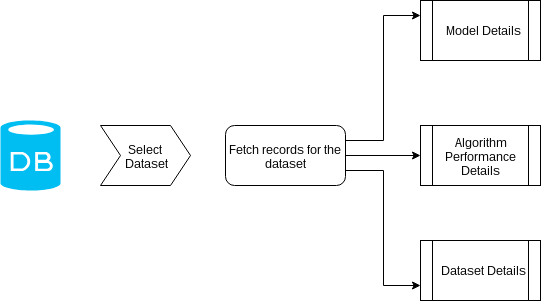
\includegraphics[width=0.8\linewidth]{thesis_template/images/Database_fetch.png}
    	\caption{Fetching Records}
    	\label{fig:fetching_records}
        \end{figure}
        



\subsection{Interpreting Results }
Figure \ref{fig:fetching_records} describes the first stage of the interface were upon selection of a dataset its records will be fetched, then the records will be processed and displayed using Dash layout rendering and html tags inside the layout. Considering future usage of the data stored in the database from the evaluation framework a certain format of attribute to values were followed in order to display the results without much processing of data when fetched from the database
The first stage of results to display is the Dataset Description with table along with performance measures and the model details from each toolkit's outcome, here for simplicity at the beginning the following attributes are displayed in the default view
Dataset Description tab
\begin{itemize}
    \item No of Instances
    \item No of features
    \item Type of task
\end{itemize}

Estimator tab for Autosklearn and Tpot
\begin{itemize}
    \item Algorithm Name
    \item Algorithm accuracy
    \item Runtime
\end{itemize}

\begin{figure}[!h]
    	\centering
    	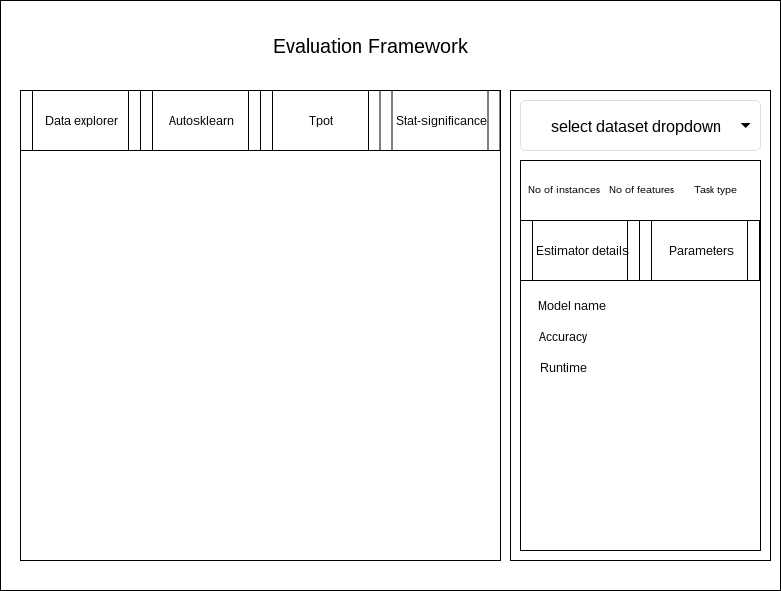
\includegraphics[width=0.8\linewidth]{thesis_template/images/Default_skeleton.png}
    	\caption{Default view skeleton}
    	\label{fig:default_skeleton}
        \end{figure}

Figure \ref{fig:default_skeleton} describes the default view of the web interface, it consists of 4 tabs on the left side and action initiator that is the select dataset from the dropdown resides on the right side with dataset's description and 2 tabs for each toolkit below
The second stage of the interface is to display the hyperparameters of each algorithms and its values as key-value pairs, this is done for both Autosklearn and Tpot since both the outcomes contain upto 100 models in combination with different hyperparameters. The third stage of the results are the statistical significance values were box-plots are drawn for both the toolkit's generated models




